\documentclass[letterpaper,10pt]{article}
\usepackage[margin=0.75in]{geometry}
\usepackage{graphicx,pdfpages,booktabs,amsmath}
\usepackage[hidelinks]{hyperref}
\pagestyle{empty}
\begin{document}
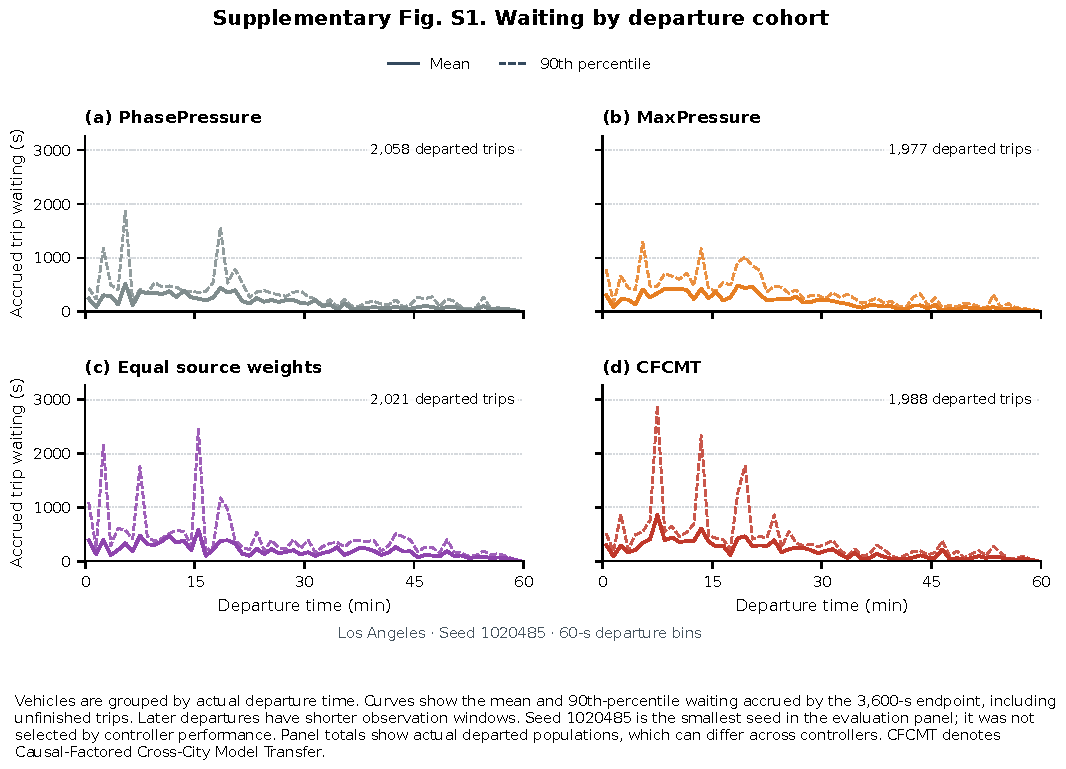
\includepdf[pages=-,scale=0.88,offset=0 2in]{Historical_supplement.pdf}
\section*{Supplementary Figure S2. Historical waiting distributions}
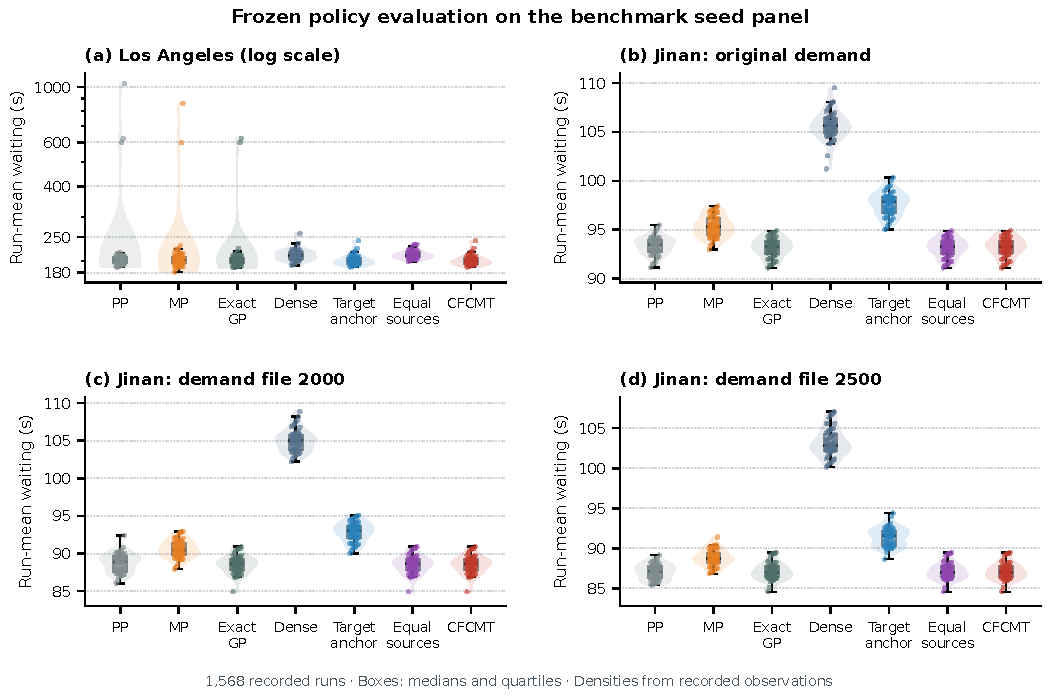
\includegraphics[width=\textwidth]{figures/fig3_benchmark_distributions.pdf}
Run-mean waiting across four scenarios and 56 reused seeds (1,568 runs). PP, MP, and GP denote PhasePressure, MaxPressure, and the exact generalized-pressure reference, respectively. Dots show run means, boxes show medians and quartiles, and violins show kernel densities. Los Angeles uses a logarithmic axis. Main-text Table IV reports the separate 896-run panel with fresh simulator seeds under the same demand profiles.
\clearpage
\section*{Supplementary Figure S3. Development-set guard comparison}
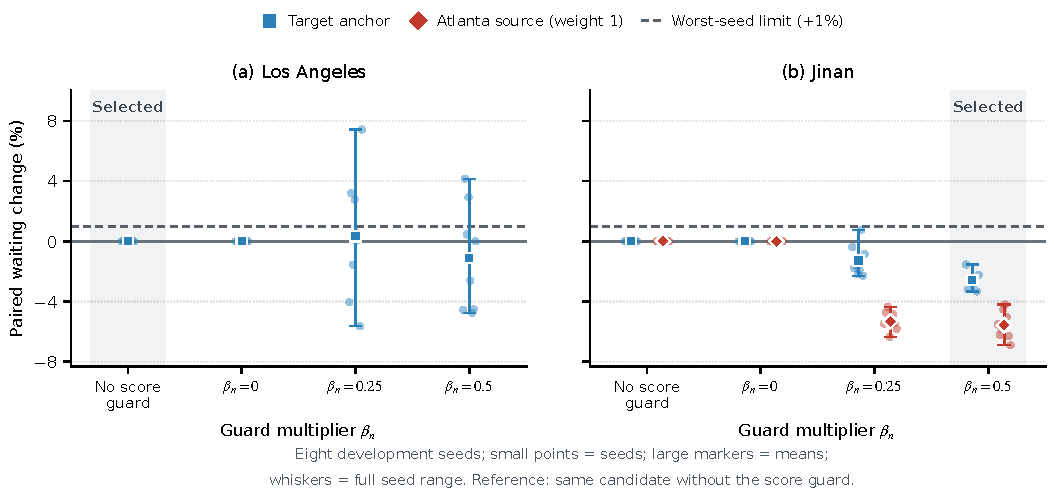
\includegraphics[width=\textwidth]{figures/fig4_guard_comparison.pdf}
Guard comparison on eight development seeds. Changes are relative to the same candidate with its score guard disabled. Dots denote seeds, large markers denote mean paired waiting changes, and whiskers show the seed range. The dashed line marks the 1\% worst-seed regression limit. Shading marks the configurations selected on the development seeds. The fresh-seed evaluation uses these frozen guard and mixture parameters.

\clearpage
\section*{Supplementary Note S1. Exploratory direct native-label transfer}
A separate development pilot tests one Cologne-to-Jinan source-label construction using 195 source action groups and 100 previously reused target challenge groups from ten seeds. Each label follows a native simulator prefix, a 10-s candidate request, and 440~s of PP continuation. For action group $g$ and candidate phase $a$, $C_g(a)$ is the mean halted vehicle count per controlled lane over 450~s. Let $a_g^{\mathrm{PP}}$ be the phase requested by PP. Training uses $[C_g(a)-C_g(a_g^{\mathrm{PP}})]L_n\times450$ halted-vehicle seconds, where $L_n$ is the controlled lane count in network $n$ (8 for the source, 144 for the target). This task differs from V93's 60-s active-plus-pending load labels and one-hour closed-loop evaluation.

Five fixed folds hold out whole target seeds. Three arms use the same 23 pre-action state and 40 candidate-minus-PP action features: target only (T), true source plus target (S), and source labels permuted within each group plus target (P). No legacy predictor outputs enter these features. All arms use the same histogram gradient-boosted squared-error regressor (100 iterations, learning rate 0.05, 15 leaves, minimum 20 rows per leaf, $L_2=10$) and total training weight 560. T allocates all weight to target rows; S and P split weight equally between source and target rows. Target demands and groups are balanced; source groups receive equal weights. Added source rows change histogram bins and leaf composition despite shared hyperparameters. Selection fixes the PP score at zero, retains the original tie rule, and forbids holding the current phase when PP requests a switch.

\begin{center}
\textbf{Table S2. Native pilot outcomes on the 100 target groups}\\[4pt]
\begin{tabular}{@{}lrrrr@{}}
\toprule
Arm & Mean cost & Overrides & Harmful overrides & Harm sum\\
\midrule
T: Target only & 1.023732 & 49 & 25 & 0.328781\\
S: True source + target & 1.024592 & 41 & 19 & 0.372160\\
P: Permuted source + target & 1.025339 & 39 & 22 & 0.400957\\
PP reference & 1.023855 & 0 & 0 & 0\\
\bottomrule
\end{tabular}
\end{center}
Harm sums are $\sum_g\max\{C_g(\widehat a_g)-C_g(a_g^{\mathrm{PP}}),0\}$, where $\widehat a_g$ is the phase selected by the arm for group $g$. Mean costs weight the ten target seeds equally. Each seed contributes four groups from the original demand profile and three from each of the 2000 and 2500 profiles. Results by demand profile and seed are available in the accompanying data.

\begin{center}
\textbf{Table S3. Source-arm paired mean-cost differences}\\[4pt]
\begin{tabular}{@{}lrr@{}}
\toprule
Comparison & Mean difference & 95\% whole-seed bootstrap interval\\
\midrule
S minus T & $+0.000859$ & $[-0.001276,\phantom{+}0.002820]$\\
S minus P & $-0.000748$ & $[-0.002079,\phantom{+}0.000880]$\\
S minus PP & $+0.000736$ & $[-0.000690,\phantom{+}0.002287]$\\
\bottomrule
\end{tabular}
\end{center}
The prespecified development gate requires all three interval upper bounds to be negative (10,000 paired seed resamples) and S's harm sum not to exceed T's. Both requirements fail: all intervals cross zero and S's harm sum increases by 13.19\%. The fixed construction is closed after 15 fits and zero new simulator trajectories, without weight, feature, or threshold reselection or expansion to new-prefix or closed-loop experiments.

\paragraph{Limitations.} The target bank is a repeatedly used model-disagreement challenge set. Shared physical units do not equate a one-intersection source with a 12-intersection target. This result evaluates one fixed source, feature set, model, and weighting; it provides neither independent transfer confirmation nor a general impossibility result. Protocol, input audit, complete scalar results, adapter, runner, and focused tests accompany this note; the original banks and frozen runtime are required to refit.

\end{document}
